% fig_fint_comparison.tex
% f_int vs I_fund showing threshold recalibration for pi-section.
% Baseline (blue solid): thresh=0.20, max_factor=5.0
% Pi-section (red dashed): thresh=0.12, max_factor=3.0
% Vertical lines at typical fault currents (alpha=0.05 and alpha=0.07)
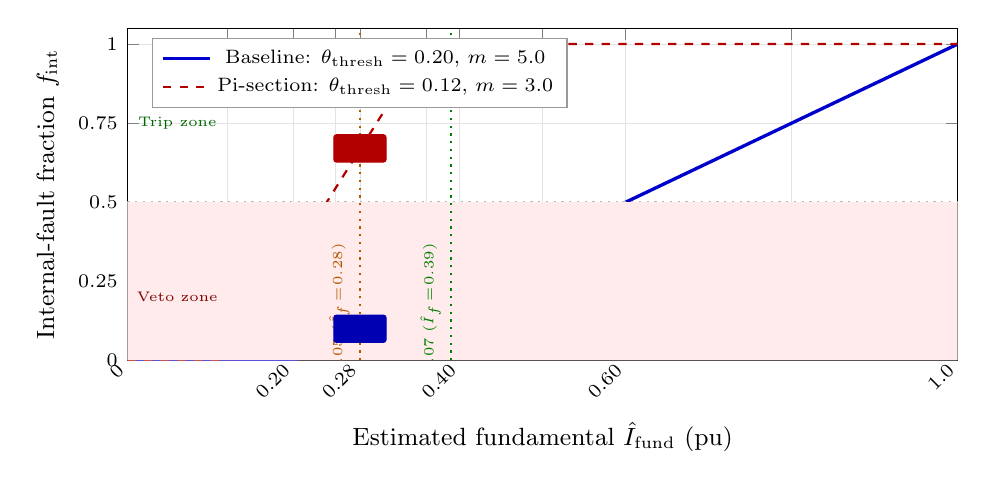
\begin{tikzpicture}
\begin{axis}[
  width=\columnwidth, height=5.8cm,
  xlabel={Estimated fundamental $\hat{I}_{\rm fund}$ (pu)},
  ylabel={Internal-fault fraction $f_{\rm int}$},
  xmin=0, xmax=1.0,
  ymin=0, ymax=1.05,
  xtick={0,0.12,0.20,0.25,0.28,0.36,0.40,0.50,0.60,0.80,1.0},
  xticklabels={0,,0.20,,0.28,,0.40,,0.60,,1.0},
  xticklabel style={rotate=45,anchor=east,font=\scriptsize},
  ytick={0,0.25,0.50,0.75,1.00},
  grid=both,
  grid style={gray!22,line width=0.3pt},
  minor grid style={gray!10},
  tick label style={font=\scriptsize},
  label style={font=\small},
  legend style={at={(0.03,0.97)},anchor=north west,
                font=\scriptsize,fill=white,draw=black!40},
  clip=true,
]

  % ---- Baseline: thresh=0.20, max_factor=5.0 ----------------------------
  % f_int = clip((I/0.20 - 1) / 4, 0, 1)
  \addplot[blue!80!black, very thick, samples=150, domain=0:1.0]
    { min( max( (x/0.20 - 1.0)/4.0, 0.0), 1.0) };
  \addlegendentry{Baseline: $\theta_{\rm thresh}=0.20$, $m=5.0$}

  % ---- Pi-section: thresh=0.12, max_factor=3.0 --------------------------
  % f_int = clip((I/0.12 - 1) / 2, 0, 1)
  \addplot[red!70!black, thick, dashed, samples=150, domain=0:1.0]
    { min( max( (x/0.12 - 1.0)/2.0, 0.0), 1.0) };
  \addlegendentry{Pi-section: $\theta_{\rm thresh}=0.12$, $m=3.0$}

  % ---- f_int = 0.50 threshold (gate veto boundary) -----------------------
  \draw[gray!55, dotted, thick]
    (axis cs:0,0.50) -- (axis cs:1.0,0.50)
    node[right, font=\tiny, gray!55]{$f_{\rm int,thresh}=0.50$};

  % ---- Veto zone (f_int < 0.50): shaded ----------------------------------
  \addplot[fill=red!8, draw=none, forget plot]
    coordinates {(0,0)(1.0,0)(1.0,0.50)(0,0.50)} \closedcycle;

  % ---- Typical fault currents -------------------------------------------
  % alpha=0.05 ag: I_fund ≈ 0.28 pu
  \draw[orange!70!black, dotted, thick]
    (axis cs:0.28, 0) -- (axis cs:0.28, 1.05)
    node[above, rotate=90, font=\tiny, orange!70!black, pos=0.10]
    {$\alpha=0.05$\;($\hat{I}_f\!=\!0.28$)};

  % alpha=0.07 ag: I_fund ≈ 0.39 pu
  \draw[green!50!black, dotted, thick]
    (axis cs:0.39, 0) -- (axis cs:0.39, 1.05)
    node[above, rotate=90, font=\tiny, green!50!black, pos=0.10]
    {$\alpha=0.07$\;($\hat{I}_f\!=\!0.39$)};

  % ---- f_int annotations at key crossings --------------------------------
  % Baseline: alpha=0.05 → f_int = (0.28/0.20-1)/4 = 0.10 (vetoed)
  \node[draw, fill=blue!8, rounded corners=1pt, font=\tiny, blue!70!black]
    at (axis cs:0.28, 0.10) {0.10};
  % Pi-section: alpha=0.05 → f_int = (0.28/0.12-1)/2 = 0.67 (not vetoed)
  \node[draw, fill=red!8, rounded corners=1pt, font=\tiny, red!70!black]
    at (axis cs:0.28, 0.67) {0.67};

  % ---- Region labels -------------------------------------------------------
  \node[font=\tiny, red!50!black] at (axis cs:0.06, 0.20) {Veto zone};
  \node[font=\tiny, green!40!black] at (axis cs:0.06, 0.75) {Trip zone};

\end{axis}
\end{tikzpicture}
